\renewcommand{\thechapter}{A}
\chapter{Anexos}

\begin{figure}[htbp]
    \centering
    \includegraphics[width=\textwidth]{img/sanger_seq.png}
    \caption[Fundamento del método de terminación de cadena (Sanger)]{Fundamento 
    del método de terminación de cadena (Sanger). Las moléculas molde/cebador se 
    mezclan con ADN polimerasa, desoxinucleótidos en exceso y didesoxinucleótidos
    (ddNTPs) marcados con fluoróforos. La polimerasa sintetiza ADN complementario 
    hasta incorporar un ddNTP, que termina la síntesis. Se genera un conjunto 
    anidado de fragmentos con diferentes longitudes, cada uno identificado por el 
    color del ddNTP terminal. Los fragmentos se separan por electroforesis de 
    alta resolución y un láser detecta el color de cada base terminal. Reproducido de 
    \cite{goldberg_genetics_2024}.}
    \label{fig:sanger_seq}
    \centering
\end{figure}

\begin{figure}[htbp]
    \centering
    \includegraphics[width=\textwidth]{img/illumina_seq.png}
    \caption[Fundamento de la secuenciación de lecturas cortas de Illumina]{
    Fundamento de la secuenciación de lecturas cortas de Illumina. En primer lugar 
    se unen adaptadores a los extremos de los fragmentos de ADN, que a su vez 
    se unen a la celda de flujo recubierta de cebadores y se amplifican mediante 
    PCR en puente para generar grupos clonales. En cada ciclo de secuenciación se 
    incorpora un nucleótido marcado con fluoróforo a las hebras en crecimiento. 
    Un láser excita los fluoróforos y un escáner óptico captura las señales de 
    cada grupo clonal. Tras la detección, se eliminan el fluoróforo y el bloqueo 
    del extremo 3' para iniciar el siguiente ciclo. La acumulación de errores de 
    sincronización (\textit{dephasing}) entre las moléculas del mismo grupo 
    clonal limita la longitud máxima de las lecturas. Reproducido de \cite{lu_next_2016}.}
    \label{fig:illumina_seq}
    \centering
\end{figure}

\begin{figure}[htbp]
    \centering
    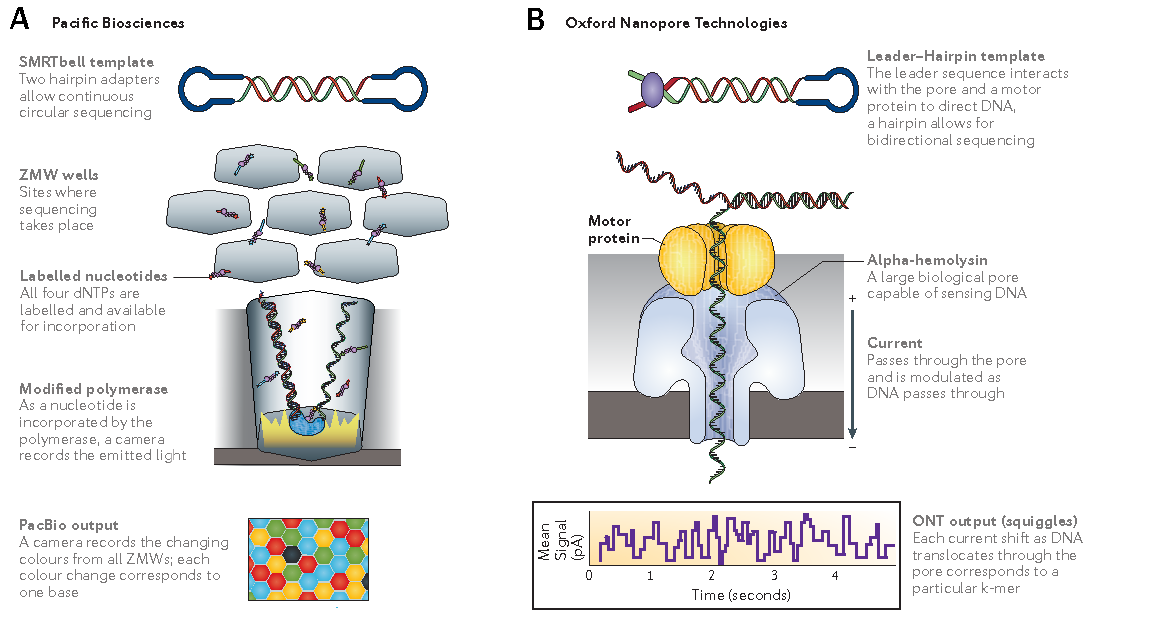
\includegraphics[width=\textwidth]{img/long_seqs.pdf}
    \caption[Fundamentos de la secuenciación de lecturas largas de PacBio y Oxford 
    Nanopore]{Fundamentos de la secuenciación de lecturas largas de PacBio y Oxford 
    Nanopore.(\textbf{A}) Secuenciación SMRT de PacBio: Las plantillas SMRTbell 
    contienen adaptadores en horquilla en ambos extremos que permiten la 
    secuenciación circular continua de ambas hebras de ADN. Estas plantillas se 
    inmovilizan en pocillos ZMW (\textit{zero-mode waveguides}) donde una 
    polimerasa modificada incorpora nucleótidos marcados con fluorescencia. 
    Durante la síntesis, una cámara registra las emisiones de luz 
    correspondientes a cada base incorporada, generando cambios de color que se 
    traducen en la secuencia de bases. (\textbf{B}) Secuenciación por nanoporos 
    de Oxford Nanopore Technologies: La plantilla de ADN contiene una secuencia 
    líder y un adaptador en horquilla que permiten la secuenciación bidireccional. 
    La secuencia líder interactúa con una proteína motora que controla la 
    translocación del ADN a través de un nanoporo biológico (alfa-hemolisina). 
    Al atravesar el poro, el ADN modula la corriente eléctrica de forma 
    específica para cada k-mero (secuencia consecutiva de k nucleótidos, 
    típicamente 5-6 bases). Las señales de salida (\textit{squiggles}) representan 
    estas modulaciones de corriente a lo largo del tiempo, que son posteriormente 
    decodificadas mediante algoritmos de basecalling para obtener la secuencia 
    de bases. Reproducido de \cite{goodwin_coming_2016}.}
    \label{fig:long_seqs}
\end{figure}

\begin{figure}[htbp]
    \centering
    \includegraphics[width=\textwidth]{img/T2T_ref.pdf}
    \caption[Huecos resueltos por el ensamblaje T2T]{Huecos resueltos por el 
    ensamblaje T2T. Cada barra representa la visualización lineal de un 
    cromosoma, con los números cromosómicos indicados a la izquierda. Los 
    segmentos rojos denotan secuencias previamente ausentes que fueron 
    resueltas por el Consorcio T2T en 2022. El cromosoma Y no está incluido, 
    ya que su compleja arquitectura, particularmente sus grandes repeticiones 
    invertidas (IRs) dispuestas en tándem, requirió análisis adicionales y fue 
    publicado de forma independiente en 2023 \cite{rhie_complete_2023}. 
    Adaptado de \cite{zahn_filling_2022}.}
    \label{fig:T2T_ref}
\end{figure}


\begin{figure}[htbp]
    \centering
    \includegraphics[width=\textwidth]{img/ont_pores.png}
    \caption[Mejoras del nanoporo R10 respecto a R9]{El diseño del nanoporo R10 
    introduce mejoras clave respecto a su predecesor R9: una estructura en barril 
    más largo y una arquitectura con doble paso de lectura. Estos cambios
    estructurales permiten una mejor resolución de regiones homopoliméricas como 
    las VNTRs, incrementando significativamente la precisión de consenso de los datos de 
    secuenciación por nanoporos. Reproducido de 
    \cite{oxford_nanopore_technologies_r103_2020}.}
    \label{fig:ont_pores}
\end{figure}


\FloatBarrier


\begingroup
\footnotesize
\begin{longtable}{>{\RaggedRight\arraybackslash}p{3.5cm} >{\RaggedRight\arraybackslash}p{9.25cm} >{\RaggedRight\arraybackslash}p{2cm}}
    \captionsetup{labelfont=bf}
    \caption[Herramientas de software utilizadas en este trabajo]{\RaggedRight Herramientas de software utilizadas en este trabajo.}\vspace{0.30cm}
    \label{tab:software}\\
    
    \toprule
\textbf{Name} & \textbf{Source} & \textbf{Reference} \\ 
\midrule
\endfirsthead

\multicolumn{3}{@{}l}{\RaggedRight \tablename\ \thetable{} -- Continued} \\
\\
\toprule
\textbf{Name} & \textbf{Source} & \textbf{Reference} \\ 
\midrule \\
\endhead \\
\midrule 
\multicolumn{3}{r}{\footnotesize Continued on next page} \\
\endfoot


\bottomrule
\endlastfoot
\\
Positron v2025.10.1-4        & \url{https://github.com/posit-dev/positron}        & --                                    \\
\\
Snakemake v9.13.5            & \url{https://github.com/snakemake/snakemake}       & \cite{koster_snakemakescalable_2012}  \\
\\
Miniforge v25.9.1            & \url{https://github.com/conda-forge/miniforge}     & --                                    \\
\\
VISOR v1.1.2.1               & \url{https://github.com/davidebolo1993/VISOR}      & \cite{bolognini_visor_2020}           \\
\\
minimap2 v2.30               & \url{https://github.com/lh3/minimap2}              & \cite{li_minimap2_2018}               \\          
\\
SAVANA v1.3.6                & \url{https://github.com/cortes-ciriano-lab/savana} & \cite{elrick_savana_2025}             \\
\\
Severus v1.6                 & \url{https://github.com/KolmogorovLab/Severus}     & \cite{keskus_severus_2025}            \\
\\
Sniffles2 v2.7.2             & \url{https://github.com/fritzsedlazeck/Sniffles}   & \cite{smolka_detection_2024}          \\
\\
SVision-Pro v2.5             & \url{https://github.com/sonGBowang125/SVision-pro} & \cite{wang_novo_2024}                 \\
\\
GW v1.2.6                    & \url{https://github.com/kcleal/gw}                 & \cite{cleal_gw_2025}                  \\
\\
UCSC Genome Browser v2025    & \url{https://genome.ucsc.edu/index.html}           & \cite{perez_ucsc_2025}                \\
\\
Wakhan v0.2.0                & \url{https://github.com/KolmogorovLab/Wakhan}      & \cite{ahmad_wakhan_2025}              \\
\\
\end{longtable}
\endgroup

\begin{figure}[htbp]
    \centering
    \includegraphics[width=\textwidth]{img/GW_UI.pdf}
    \caption[Inspección de alineamientos para validación de SVs con GW]{Inspección de alineamientos 
    para validación de SVs con GW. La herramienta se lanza a través de la 
    terminal, solicitando inicialmente la selección del genoma de referencia 
    (\textbf{a}) y abriendo una ventana gráfica vacía. La carga de archivos BAM y 
    VCF que contienen SVs mediante arrastre a la ventana gráfica genera una 
    cuadrícula de imágenes en miniatura correspondientes a los puntos de ruptura 
    indicados en el VCF (\textbf{b}). Al pasar el cursor sobre una imagen se 
    muestran las coordenadas del punto de ruptura en la terminal, mientras que 
    al hacer clic se abre una vista detallada del alineamiento con capacidades 
    de navegación a lo largo del cromosoma (\textbf{c}). El usuario puede
    regresar a la cuadrícula de imágenes y alternar botones Verdadero/Falso en 
    las esquinas inferiores izquierdas para rastrear el estado de validación de 
    las SVs, el cual puede exportarse como una lista para análisis posteriores.}
    \label{fig:GW_UI}
\end{figure}

\newpage

\begingroup
\footnotesize
\begin{longtable}{>{\RaggedRight\arraybackslash}p{3.5cm} >{\RaggedRight\arraybackslash}p{2cm} >{\RaggedRight\arraybackslash}p{2cm} >{\RaggedRight\arraybackslash}p{2cm}}
\captionsetup{labelfont=bf}
\caption[Tamaños de archivos por longitud de lectura]{\RaggedRight Tamaño en gigabytes de archivos de secuenciación de lecturas largas generados con VISOR toolkit a diferentes longitudes de lectura. Los archivos incluyen BAM, sus índices (BAI), y lecturas no alineadas en archivos FASTQ.}\vspace{0.30cm}
\label{tab:file_sizes}\\
\toprule
\textbf{Longitud de lectura} & \textbf{BAM} & \textbf{BAI} & \textbf{FASTQ} \\ 
\midrule
\endfirsthead
\multicolumn{4}{@{}l}{\RaggedRight \tablename\ \thetable{} -- Continuación} \\
\\
\toprule
\textbf{Longitud de lectura} & \textbf{BAM} & \textbf{BAI} & \textbf{FASTQ} \\ 
\midrule \\
\endhead \\
\midrule 
\multicolumn{4}{r}{\footnotesize Continúa en la página siguiente} \\
\endfoot
\bottomrule
\endlastfoot
\\
15000\_normal & 163.88 & 0.0521 & 129.32 \\
\\
15000 & 161.36 & 0.0513 & 127.14 \\
\\
15000 & 161.30 & 0.0513 & 127.15 \\
\\
15000 & 161.22 & 0.0513 & 127.14 \\
\\
30000\_normal & 159.51 & 0.0142 & 127.96 \\
\\
30000 & 156.75 & 0.0140 & 125.79 \\
\\
30000 & 156.79 & 0.0140 & 125.79 \\
\\
30000 & 156.98 & 0.0140 & 125.79 \\
\\
50000\_normal & 157.58 & 0.0091 & 125.85 \\
\\
50000 & 154.63 & 0.0089 & 123.72 \\
\\
50000 & 154.66 & 0.0089 & 123.73 \\
\\
50000 & 154.52 & 0.0089 & 123.73 \\
\\
100000\_normal & 162.33 & 0.0075 & 122.89 \\
\\
100000 & 159.78 & 0.0074 & 120.80 \\
\\
100000 & 159.46 & 0.0074 & 120.80 \\
\\
100000 & 160.12 & 0.0074 & 120.80 \\
\\
\midrule
\textbf{Total} & 2540.86 & 0.3277 & 1998.41 \\
\end{longtable}
\endgroup

\begin{figure}[htbp]
    \centering
    \includegraphics[width=\textwidth]{data/cluster_bmk/calls_data/chr1_del1q21.pdf}
    \caption[Breakpoints de la duplicación en tándem de 1q21 visualizados en GW]{Breakpoints 
    de la duplicación en tándem de 1q21 visualizados en GW. De arriba a abajo: 
    genoma de referencia con barra de escala, posiciones de los breakpoints (marcados con 
    triángulos invertidos), histograma de cobertura de secuenciación (el gris indica 
    concordancia con la referencia), lecturas alineadas, e ideograma del cromosoma 
    (la marca vertical roja señala la región visualizada). Los datos corresponden 
    a la muestra tumoral A con longitud media de lectura de 15 kb.}
    \label{fig:chr1_del1q21}
\end{figure}

\begin{figure}[htbp]
    \centering
    \includegraphics[width=\textwidth]{data/cluster_bmk/calls_data/chr6_inv6q25.1.pdf}
    \caption[Breakpoints de la inversión cromosómica de 6q25.1 visualizados en GW]{Breakpoints 
    de la inversión cromosómica de 6q25.1 visualizados en GW. De arriba a abajo: 
    genoma de referencia con barra de escala, posiciones de los breakpoints (marcados con 
    triángulos invertidos), histograma de cobertura de secuenciación (el gris indica 
    concordancia con la referencia), lecturas alineadas, e ideograma del cromosoma 
    (la marca vertical roja señala la región visualizada). Los datos corresponden 
    a la muestra tumoral A con longitud media de lectura de 15 kb.}
    \label{fig:chr6_inv6q25.1}
\end{figure}

\begin{figure}[htbp]
    \centering
    \includegraphics[width=\textwidth]{data/cluster_bmk/calls_data/chr9_del9p21.3.pdf}
    \caption[Breakpoints de la translocación cromosómica de cortar-pegar en 9p21.3 
    visualizados en GW]{Breakpoints de la translocación cromosómica de cortar-pegar en 9p21.3 
    visualizados en GW. De arriba a abajo: genoma de referencia con barra de escala, posiciones 
    de los breakpoints (marcados con triángulos invertidos), histograma de cobertura 
    de secuenciación (el gris indica concordancia con la referencia), lecturas 
    alineadas, e ideograma del cromosoma (la marca vertical roja señala la región 
    visualizada). Los datos corresponden a la muestra tumoral A con longitud media 
    de lectura de 15 kb.}
    \label{fig:chr9_del9p21.3}
\end{figure}

\begin{sidewaysfigure}
    \centering
    \begin{subfigure}[b]{0.48\textwidth}
        \centering
        \caption*{\textbf{a}}
        \includegraphics[width=\textwidth]{data/cluster_bmk/calls_data/chr11-14_A.pdf}
        \label{fig:chr11-14_A}
    \end{subfigure}
    \hfill
    \begin{subfigure}[b]{0.48\textwidth}
        \centering
        \caption*{\textbf{b}}
        \includegraphics[width=\textwidth]{data/cluster_bmk/calls_data/chr11-14_B.pdf}
        \label{fig:chr11-14_B}
    \end{subfigure}
    
    \begin{subfigure}[b]{0.48\textwidth}
        \centering
        \caption*{\textbf{c}}
        \includegraphics[width=\textwidth]{data/cluster_bmk/calls_data/chr11-14_C.pdf}
        \label{fig:chr11-14_C}
    \end{subfigure}
    \hfill
    \begin{subfigure}[b]{0.48\textwidth}
        \centering
        \caption*{\textbf{d}}
        \includegraphics[width=\textwidth]{data/cluster_bmk/calls_data/chr11-14_D.pdf}
        \label{fig:chr11-14_D}
    \end{subfigure}
    \caption[Breakpoints de la translocación recíproca entre 14q32 y 11q13 
    visualizados en GW]{Breakpoints de la translocación recíproca entre 14q32 y 11q13 
    visualizados en GW. (a) y (b) muestran los breakpoints en el cromosoma 11, 
    (c) y (d) muestran los breakpoints en el cromosoma 14. En cada panel, de arriba 
    a abajo: genoma de referencia con barra de escala, posiciones de los breakpoints 
    (marcados con triángulos invertidos), histograma de cobertura de secuenciación 
    (el gris indica concordancia con la referencia), lecturas alineadas, e ideograma 
    del cromosoma (la marca vertical roja señala la región visualizada). Los datos 
    corresponden a la muestra tumoral A con longitud media de lectura de 15 kb.}
    \label{fig:chr11-14_translocation}
\end{sidewaysfigure}

\begin{figure}[htbp]
    \centering
    \includegraphics[width=\textwidth]{data/cluster_bmk/calls_data/chr17_del17p13.pdf}
    \caption[Breakpoints de la deleción de 17p13 visualizados en GW]{Breakpoints 
    de la deleción de 17p13 visualizados en GW. De arriba a abajo: genoma de 
    referencia con barra de escala, posiciones de los breakpoints (marcados con 
    triángulos invertidos), histograma de cobertura de secuenciación (el gris 
    indica concordancia con la referencia), lecturas alineadas, e ideograma del 
    cromosoma (la marca vertical roja señala la región visualizada). Los datos 
    corresponden a la muestra tumoral A con longitud media de lectura de 15 kb.}
    \label{fig:chr17_del17p13}
\end{figure}

\begin{figure}[htbp]
    \centering
    \includegraphics[width=\textwidth]{img/FISH&CNAs.pdf}
    \caption[Análisis de CNAs de un paciente diagnosticado de mieloma 
    múltiple mediante FISH y secuenciación de lecturas largas]{Análisis de CNAs 
    de un paciente diagnosticado de MM mediante FISH y secuenciación 
    de lecturas largas. (\textbf{A}) Imágenes representativas de FISH realizadas por el 
    personal clínico del Hospital 12 de Octubre que revelan un cariotipo complejo 
    característico de MM: (\textbf{AI}) las sondas específicas de locus (LSI, \textit{Locus-Specific 
    Identifier}) 1q21(\textit{CSF1R})/1p32(\textit{CDKN2C}) detectan ganancia en el número de 
    copias de la región 1p32 (rojo) y número de copias normal de 1q21 (verde); 
    (\textbf{AII}) las sondas XL de tres colores para los genes del cromosoma 13 (\textit{RB1, 
    DLEU, LAMP}) confirman su monosomía; (\textbf{AIII}) sondas LSI 17q22 (\textit{TP53/MPO}) 
    muestran la pérdida de una copia de TP53 (verde) y ganancia de múltiples 
    copias de \textbf{MPO} (rojo). (\textbf{B}) Perfil genómico de número de copias obtenido 
    mediante secuenciación, los recuadros negros indican las regiones cromosómicas 
    correspondientes a las sondas FISH mostradas previamente, mientras que el recuadro 
    morado en línea discontinua señala una disomía uniparental del 4p. Las nubes de 
    puntos rojos y azules representan la profundidad de lectura por bin para los 
    haplotipos HP-1 y HP-2, respectivamente; las líneas horizontales indican números enteros de 
    copias. El paciente presenta alteraciones cromosómicas extensas, incluyendo 
    ganancias (+1q, +3, +4, +15 y +17q) y pérdidas (del 13, del 17p y del 20p), consistentes con el 
    cariotipo complejo típico de MM. Datos provenientes de investigación 
    propia \cite{haertle_multi-omic_2026}}
    \label{fig:FISH_and_CNAs}
\end{figure}